\documentclass[12pt]{report} %fuente a 12pt

% MÁRGENES: 2,5 cm sup. e inf.; 3 cm izdo. y dcho.
\usepackage[
a4paper,
vmargin=2.5cm,
hmargin=3cm
]{geometry}

% INTERLINEADO: Estrecho (6 ptos./interlineado 1,15) o Moderado (6 ptos./interlineado 1,5)
\renewcommand{\baselinestretch}{1.15}
\parskip=6pt

% DEFINICIÓN DE COLORES para portada y listados de código
\usepackage[table]{xcolor}
\definecolor{azulUC3M}{RGB}{0,0,102}
\definecolor{gray97}{gray}{.97}
\definecolor{gray75}{gray}{.75}
\definecolor{gray45}{gray}{.45}

% Soporte para GENERAR PDF/A
\usepackage[a-1b]{pdfx}

% ENLACES
\usepackage{hyperref}
\hypersetup{colorlinks=true,
	linkcolor=black, % enlaces a partes del documento (p.e. índice) en color negro
	urlcolor=blue} % enlaces a recursos fuera del documento en azul

\usepackage{pdfpages}

% EXPRESIONES MATEMATICAS
\usepackage{amsmath,amssymb,amsfonts,amsthm}

\usepackage{txfonts} 
\usepackage[T1]{fontenc}
\usepackage[utf8]{inputenc}

\usepackage{tikz}
\usepackage{pgfplots}

\usepackage[spanish, es-tabla]{babel} 
\usepackage[babel, spanish=spanish]{csquotes}
\AtBeginEnvironment{quote}{\small}

% diseño de PIE DE PÁGINA
\usepackage{fancyhdr}
\pagestyle{fancy}
\fancyhf{}
\renewcommand{\headrulewidth}{0pt}
\rfoot{\thepage}
\fancypagestyle{plain}{\pagestyle{fancy}}

% DISEÑO DE LOS TÍTULOS de las partes del trabajo (capítulos y epígrafes o subcapítulos)
\usepackage{titlesec}
\usepackage{titletoc}
\titleformat{\chapter}[block]
{\large\bfseries\filcenter}
{\thechapter.}
{5pt}
{\MakeUppercase}
{}
\titlespacing{\chapter}{0pt}{0pt}{*3}
\titlecontents{chapter}
[0pt]                                               
{}
{\contentsmargin{0pt}\thecontentslabel.\enspace\uppercase}
{\contentsmargin{0pt}\uppercase}                        
{\titlerule*[.7pc]{.}\contentspage}                 

\titleformat{\section}
{\bfseries}
{\thesection.}
{5pt}
{}
\titlecontents{section}
[5pt]                                               
{}
{\contentsmargin{0pt}\thecontentslabel.\enspace}
{\contentsmargin{0pt}}
{\titlerule*[.7pc]{.}\contentspage}

\titleformat{\subsection}
{\normalsize\bfseries}
{\thesubsection.}
{5pt}
{}
\titlecontents{subsection}
[10pt]                                               
{}
{\contentsmargin{0pt}                          
	\thecontentslabel.\enspace}
{\contentsmargin{0pt}}                        
{\titlerule*[.7pc]{.}\contentspage}  


% DISEÑO DE TABLAS.
\usepackage{multirow} % permite combinar celdas 
\usepackage{caption} % para personalizar el título de tablas y figuras
\usepackage{floatrow} % utilizamos este paquete y sus macros \ttabbox y \ffigbox para alinear los nombres de tablas y figuras de acuerdo con el estilo definido. Para su uso ver archivo de ejemplo 
\usepackage{array} % con este paquete podemos definir en la siguiente línea un nuevo tipo de columna para tablas: ancho personalizado y contenido centrado
\newcolumntype{P}[1]{>{\centering\arraybackslash}p{#1}}
\DeclareCaptionFormat{upper}{#1#2\uppercase{#3}\par}

% Diseño de tabla para ingeniería
\captionsetup[table]{
	format=upper,
	name=TABLA,
	justification=centering,
	labelsep=period,
	width=.75\linewidth,
	labelfont=small,
	font=small,
}

% DISEÑO DE FIGURAS.
\usepackage{graphicx}
\graphicspath{{img/}} %ruta a la carpeta de imágenes

% Diseño de figuras para ingeniería
\captionsetup[figure]{
	format=hang,
	name=Fig.,
	singlelinecheck=off,
	labelsep=period,
	labelfont=small,
	font=small		
}

% NOTAS A PIE DE PÁGINA
\usepackage{chngcntr} %para numeración contínua de las notas al pie
\counterwithout{footnote}{chapter}

% LISTADOS DE CÓDIGO
% soporte y estilo para listados de código. Más información en https://es.wikibooks.org/wiki/Manual_de_LaTeX/Listados_de_código/Listados_con_listings
\usepackage{listings}

% definimos un estilo de listings
\lstdefinestyle{estilo}{ frame=Ltb,
	framerule=0pt,
	aboveskip=0.5cm,
	framextopmargin=3pt,
	framexbottommargin=3pt,
	framexleftmargin=0.4cm,
	framesep=0pt,
	rulesep=.4pt,
	backgroundcolor=\color{gray97},
	rulesepcolor=\color{black},
	%
	basicstyle=\ttfamily\footnotesize,
	keywordstyle=\bfseries,
	stringstyle=\ttfamily,
	showstringspaces = false,
	commentstyle=\color{gray45},     
	%
	numbers=left,
	numbersep=15pt,
	numberstyle=\tiny,
	numberfirstline = false,
	breaklines=true,
	xleftmargin=\parindent
}

\captionsetup[lstlisting]{font=small, labelsep=period}
% fijamos el estilo a utilizar 
\lstset{style=estilo}
\renewcommand{\lstlistingname}{\uppercase{Código}}

\pgfplotsset{compat=1.17} 
%-------------
%	DOCUMENTO
%-------------

\begin{document}
\pagenumbering{roman} % Se utilizan cifras romanas en la numeración de las páginas previas al cuerpo del trabajo
	
%----------
%	PORTADA
%----------	
\begin{titlepage}
	\begin{sffamily}
	\color{azulUC3M}
	\begin{center}
		\begin{figure}[H] %incluimos el logotipo de la Universidad
			\makebox[\textwidth][c]{
\includegraphics[width=16cm]{Portada_Logo.png}}
		\end{figure}
		\vspace{2.5cm}
		\begin{Large}
			Grado en Ingeniería Informática\\			
			2018-2019\\
			\vspace{2cm}		
			\textsl{Apuntes}\\
			\bigskip
		\end{Large}
		 	{\Huge Programación}\\
		 	\vspace*{0.5cm}
	 		\rule{10.5cm}{0.1mm}\\
			\vspace*{0.9cm}
			{\LARGE Jorge Rodríguez Fraile\footnote{\href{mailto:100405951@alumnos.uc3m.es}{Universidad: 100405951@alumnos.uc3m.es}  |  \href{mailto:jrf1616@gmail.com}{Personal: jrf1616@gmail.com}}}\\ 
			\vspace*{1cm}
	\end{center}
	\vfill
	\color{black}
		
\includegraphics[width=4.2cm]{img/creativecommons.png}\\
		Esta obra se encuentra sujeta a la licencia Creative Commons\\ \textbf{Reconocimiento - No Comercial - Sin Obra Derivada}
	\end{sffamily}
\end{titlepage}

%----------
%	ÍNDICES
%----------	

%--
% Índice general
%-
\tableofcontents
\thispagestyle{fancy}

%--
% Índice de figuras. Si no se incluyen, comenta las líneas siguientes
%-
%\listoffigures
%\thispagestyle{fancy}

%--
% Índice de tablas. Si no se incluyen, comenta las líneas siguientes
%-
%\listoftables
%\thispagestyle{fancy}

%----------
%	TRABAJO
%----------	
\clearpage
\pagenumbering{arabic} % numeración con múmeros arábigos para el resto de la publicación	


%----------
%	COMENZAR A ESCRIBIR AQUI
%----------	


\part{Presentación de la Asignatura}

\includepdf[pages=-]{docs/0._Presentacion_de_la_Asignatura.pdf}

\part{Introducción a la Programación}
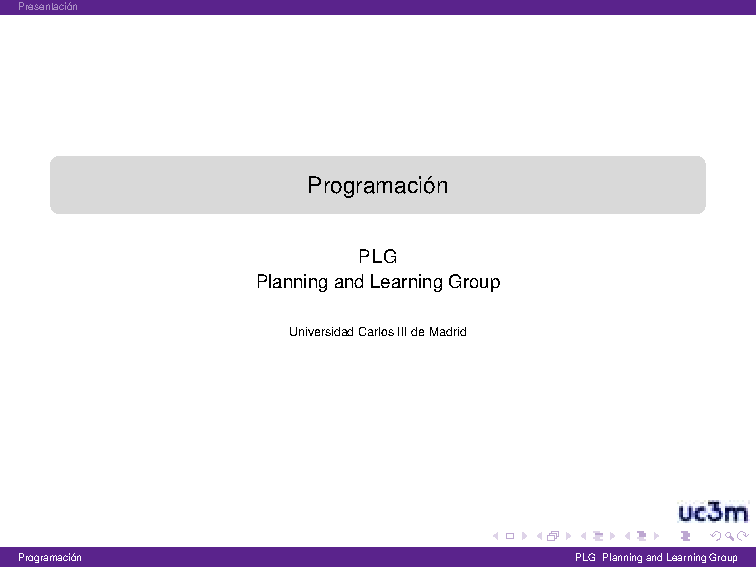
\includepdf[pages=-]{docs/1._Introduccion_a_la_Programacion.pdf}
\includepdf[pages=-]{docs/Practica_Semanal_1_Algoritmos.pdf}

\part{Diagramas de Flujo}

\includepdf[pages=-]{docs/2._Diagramas_de_Flujo.pdf}

\includepdf[pages=-]{docs/Semana_2.pdf}

\part{Introdución a Java}
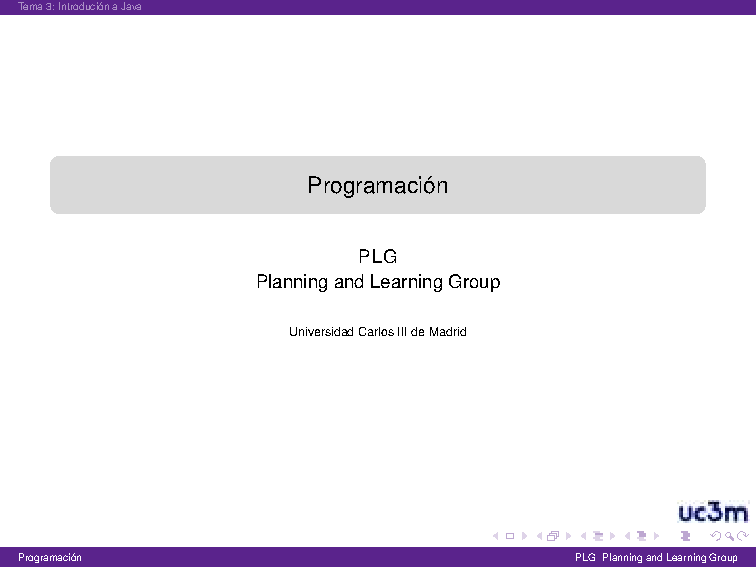
\includepdf[pages=-]{docs/3._Introducion_a_Java.pdf}
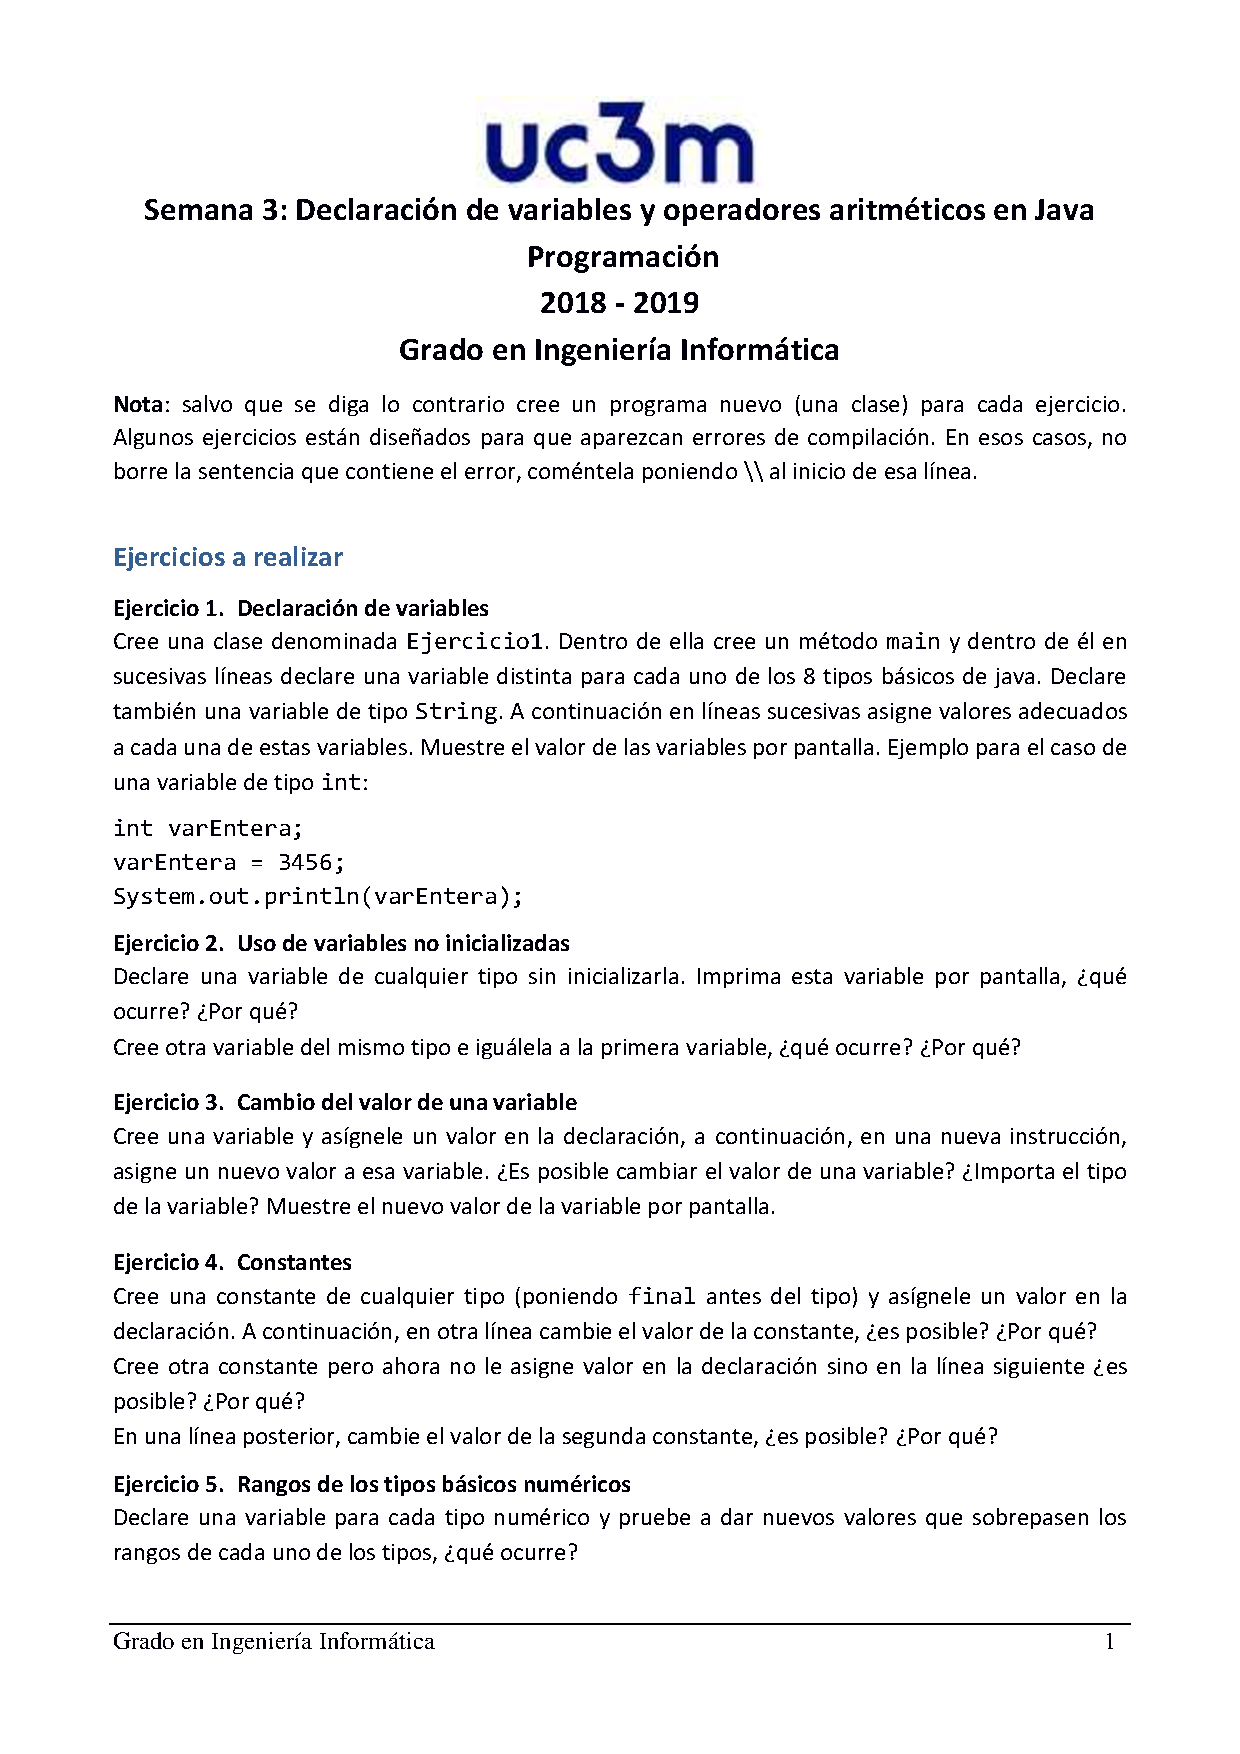
\includepdf[pages=-]{docs/Ejercicios-Semana-03-Variables_y_operadores_18-19.pdf}

\part{Condicionales y bucles}
\includepdf[pages=-]{docs/4._Condicionales_y_bucles.pdf}
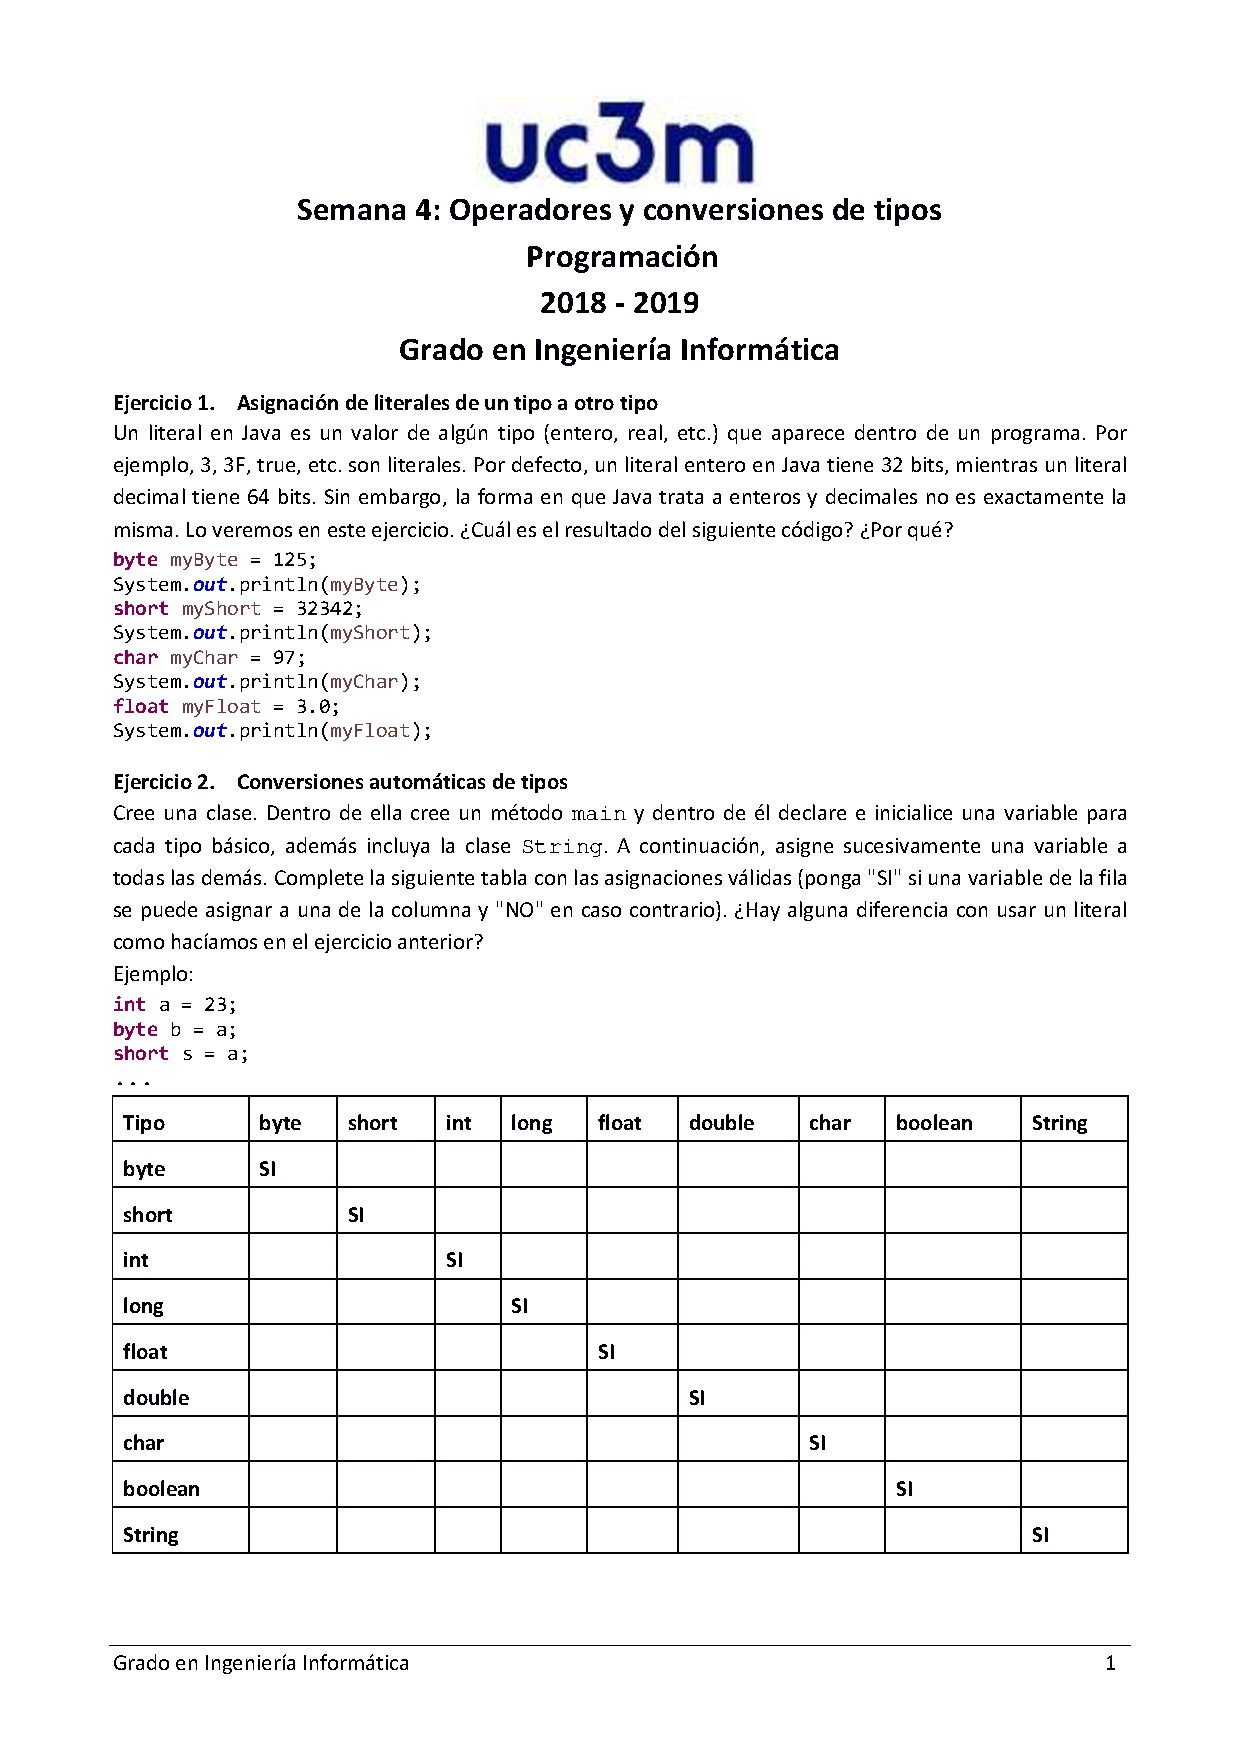
\includepdf[pages=-]{docs/Semana_4_Operadores_y_Casting.pdf}

\part{Estructuras de datos sencillas}
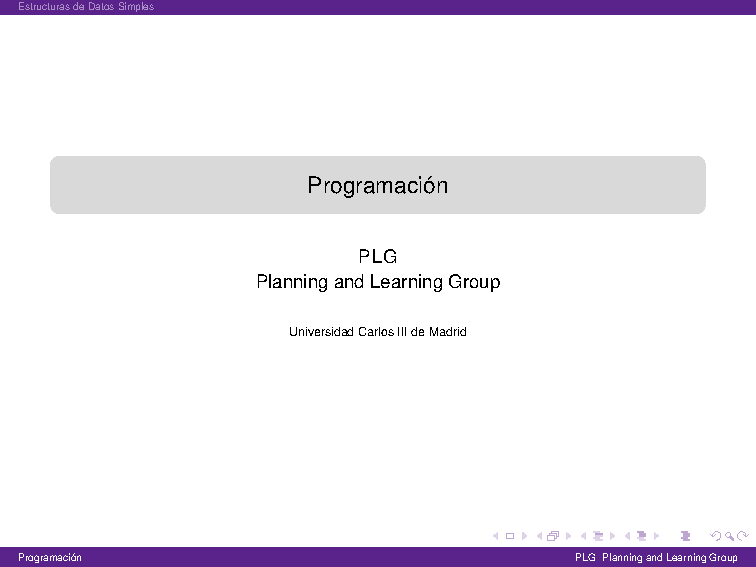
\includepdf[pages=-]{docs/5._Estructuras_de_datos_sencillas.pdf}

\includepdf[pages=-]{docs/Semana_5_Condicionales.pdf}

\part{Clases, objetos y métodos}
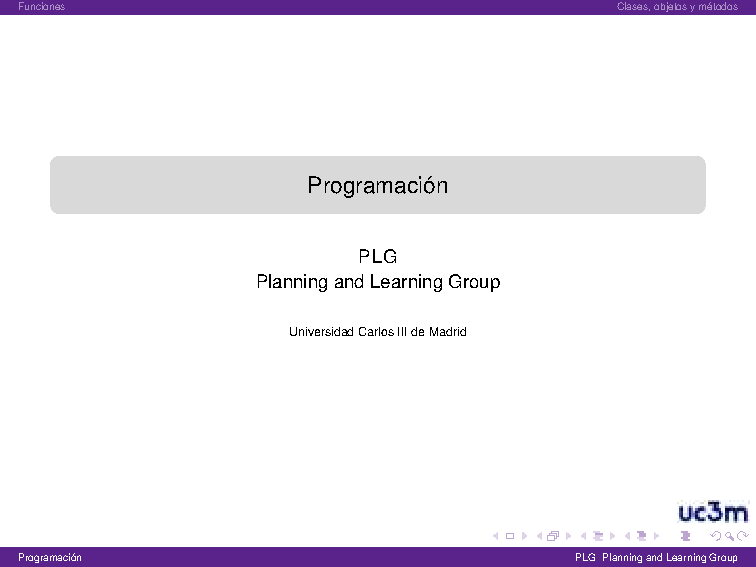
\includepdf[pages=-]{docs/6._Clases_objetos_y_metodos.pdf}
\includepdf[pages=-]{docs/Bucles.pdf}

\part{Clases útiles (Scanner, String, Envoltorios y Math}
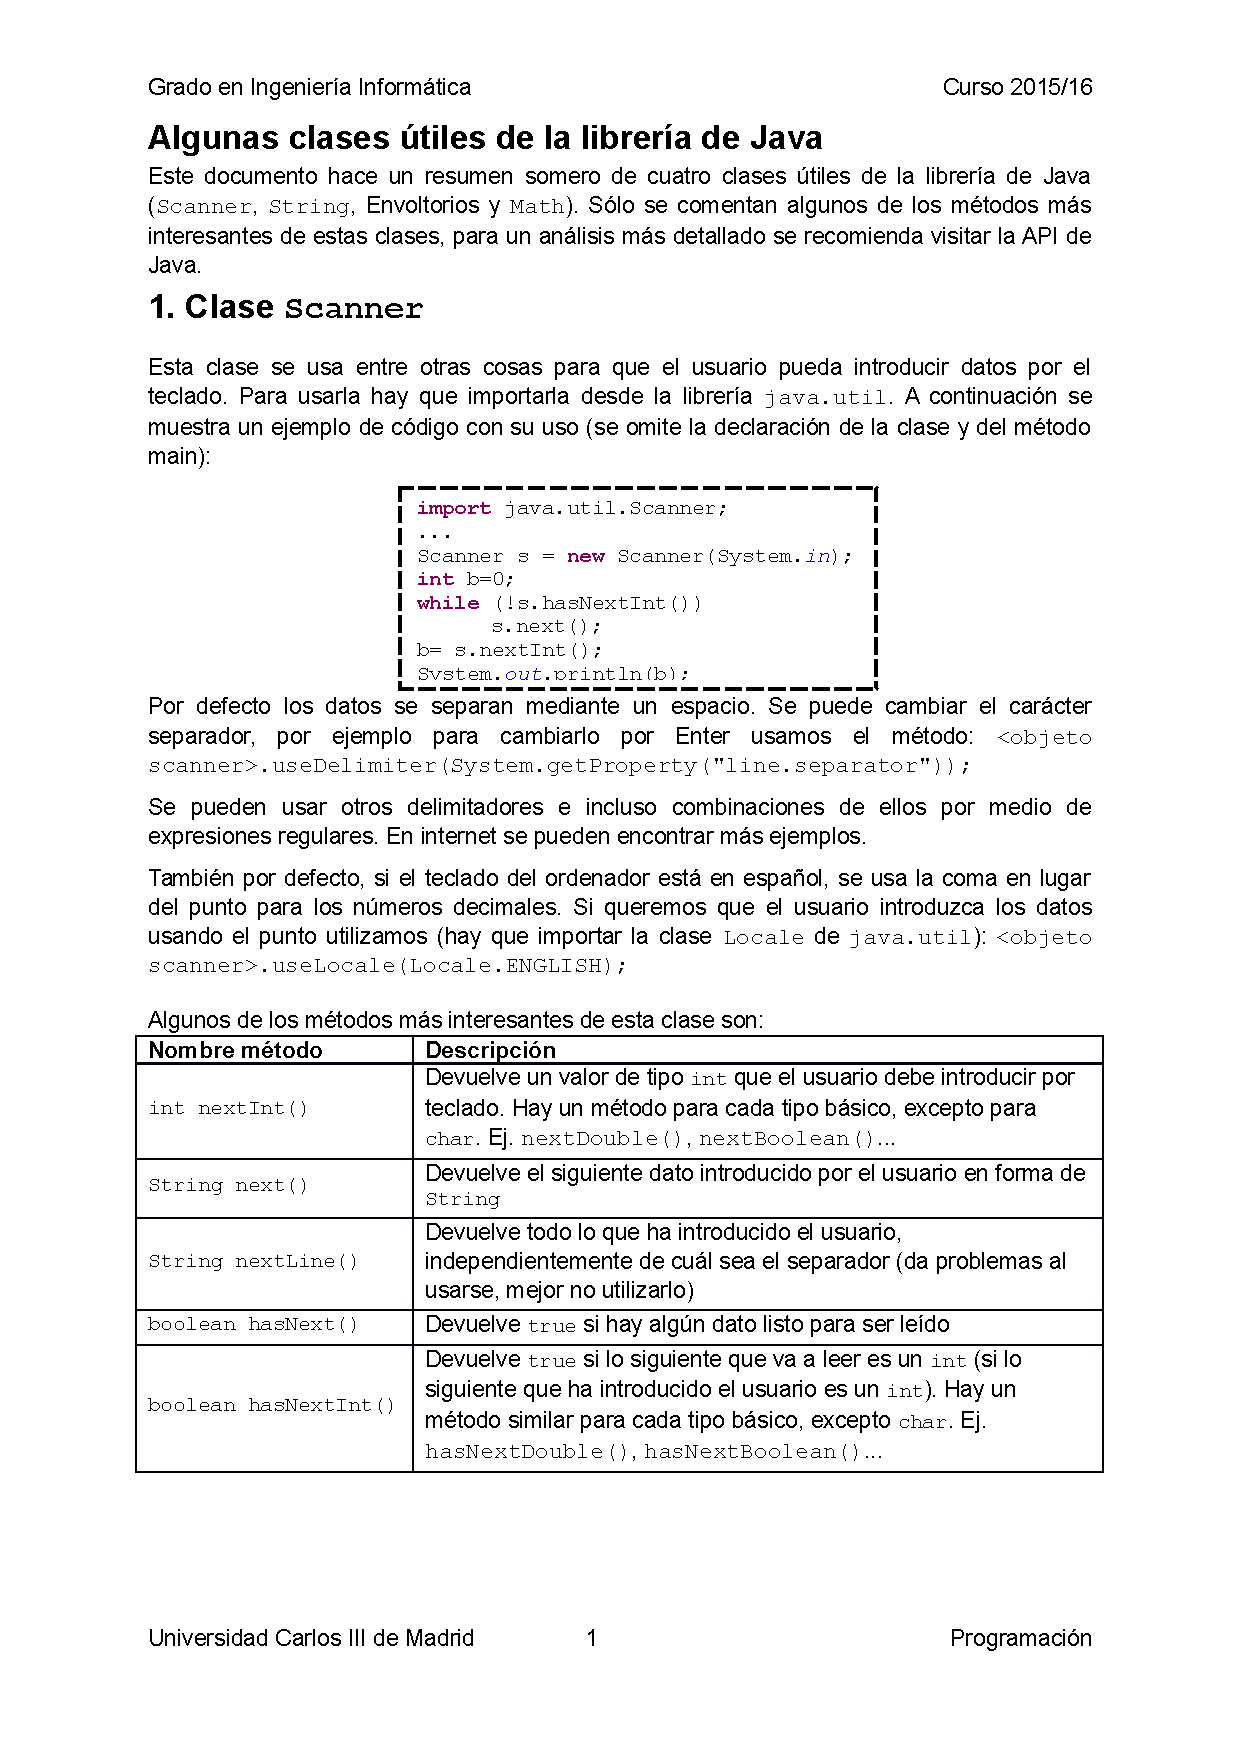
\includepdf[pages=-]{docs/7._Clases_utiles_(Scanner_String_Envoltorios_y_Math).pdf}

\includepdf[pages=-]{docs/Arrays_Semana_7.pdf}

\part{Más POO - Herencia y Polimorfismo}
\includepdf[pages=-]{docs/8._Mas_POO_-_Herencia_y_Polimorfismo.pdf}

\includepdf[pages=-]{docs/Semana_09.pdf}

\part{Algoritmos sobre listas}
\includepdf[pages=-]{docs/9._Algoritmos_sobre_listas.pdf}
\includepdf[pages=-]{docs/Ejercicio_Semana_10_Objetos-Metodos.pdf}

\includepdf[pages=-]{docs/Ejercicios-Semana-11-MetodosIII_y_Strings.pdf}
\includepdf[pages=-]{docs/Semana_12_Metodos_generales.pdf}

\includepdf[pages=-]{docs/MemoriaGalaga-mae-jrf.pdf}

\part{Exámenes}
\includepdf[pages=-]{docs/11-12-Parcial.pdf}
\includepdf[pages=-]{docs/89-Partial_Exam-13-14-Solved.pdf}
\includepdf[pages=-]{docs/Partial_2017-2018.pdf}
\includepdf[pages=-]{docs/prueba1_nov_08_61-62-Soluciones.pdf}
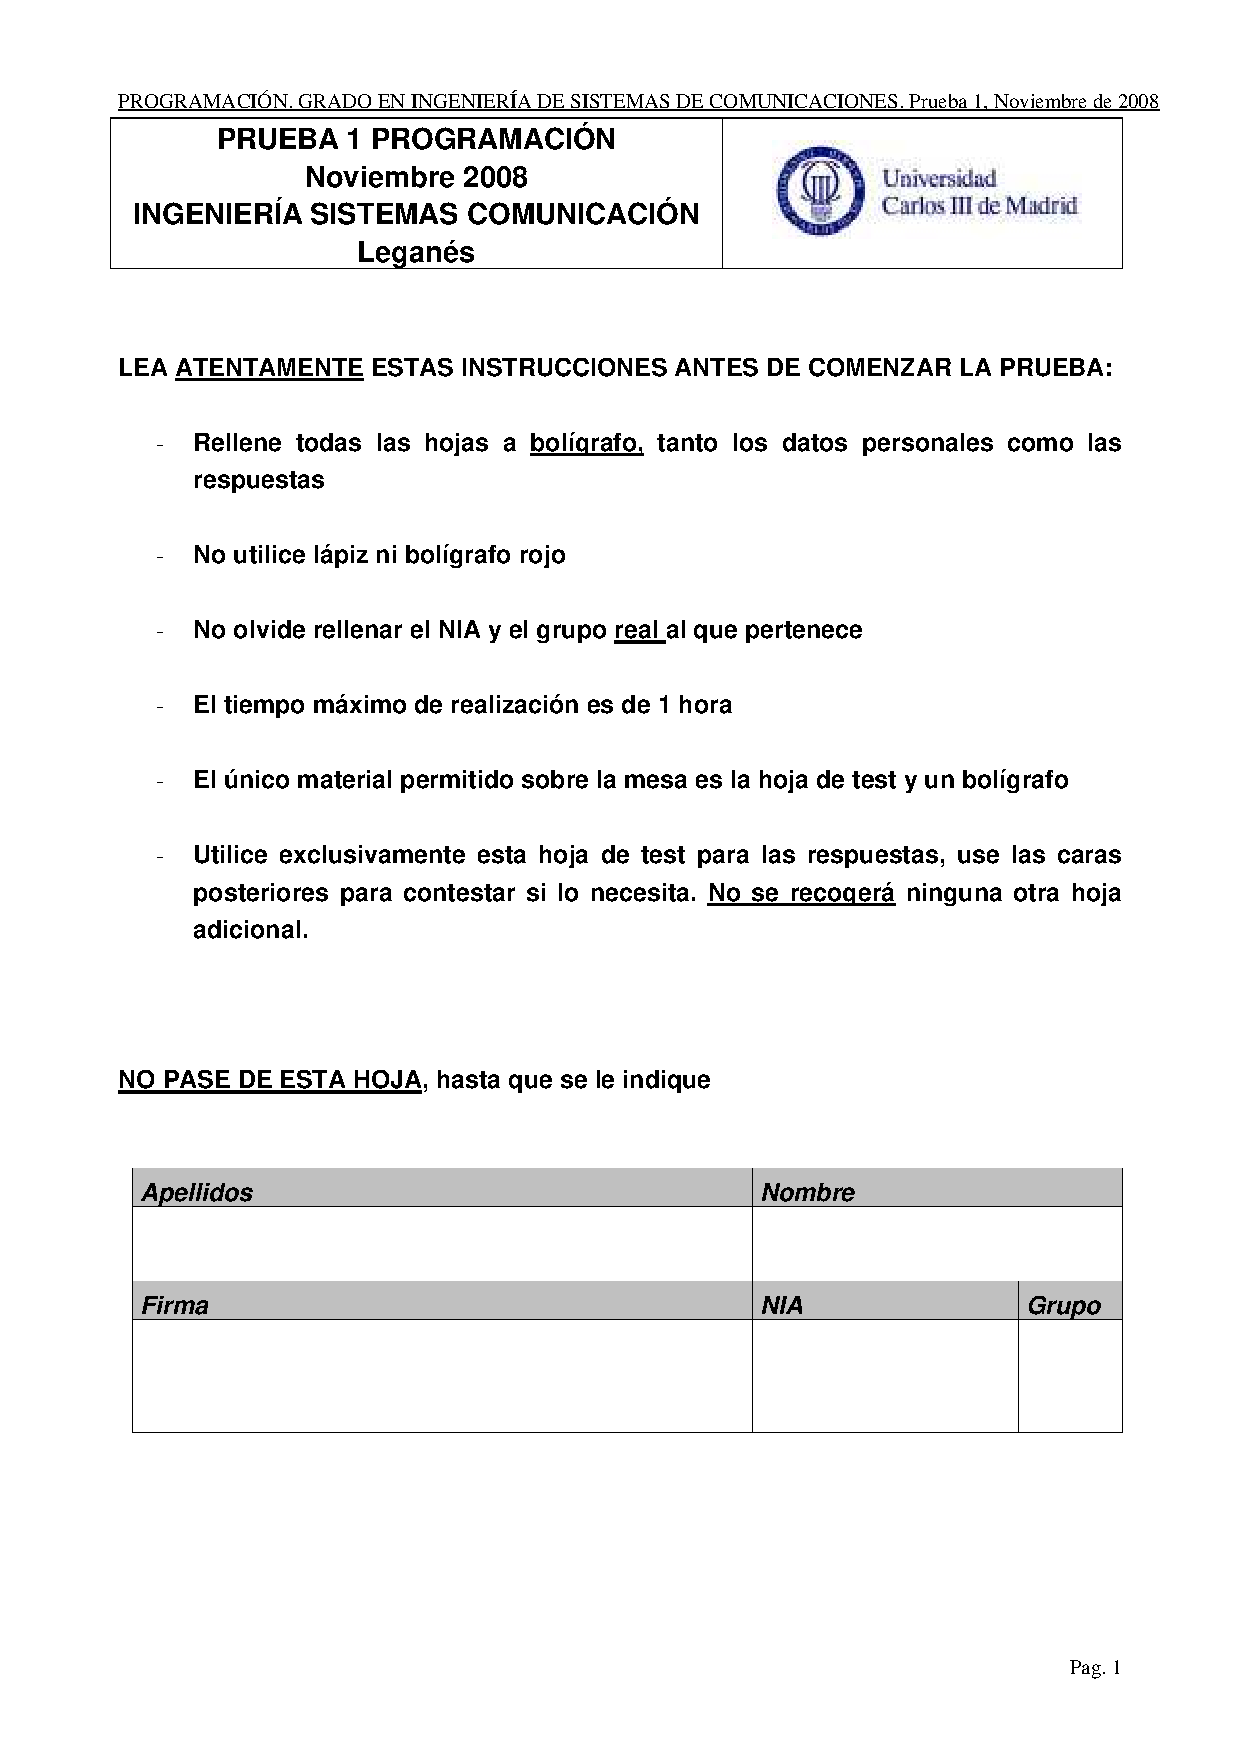
\includepdf[pages=-]{docs/prueba1_nov_08_61-62.pdf}
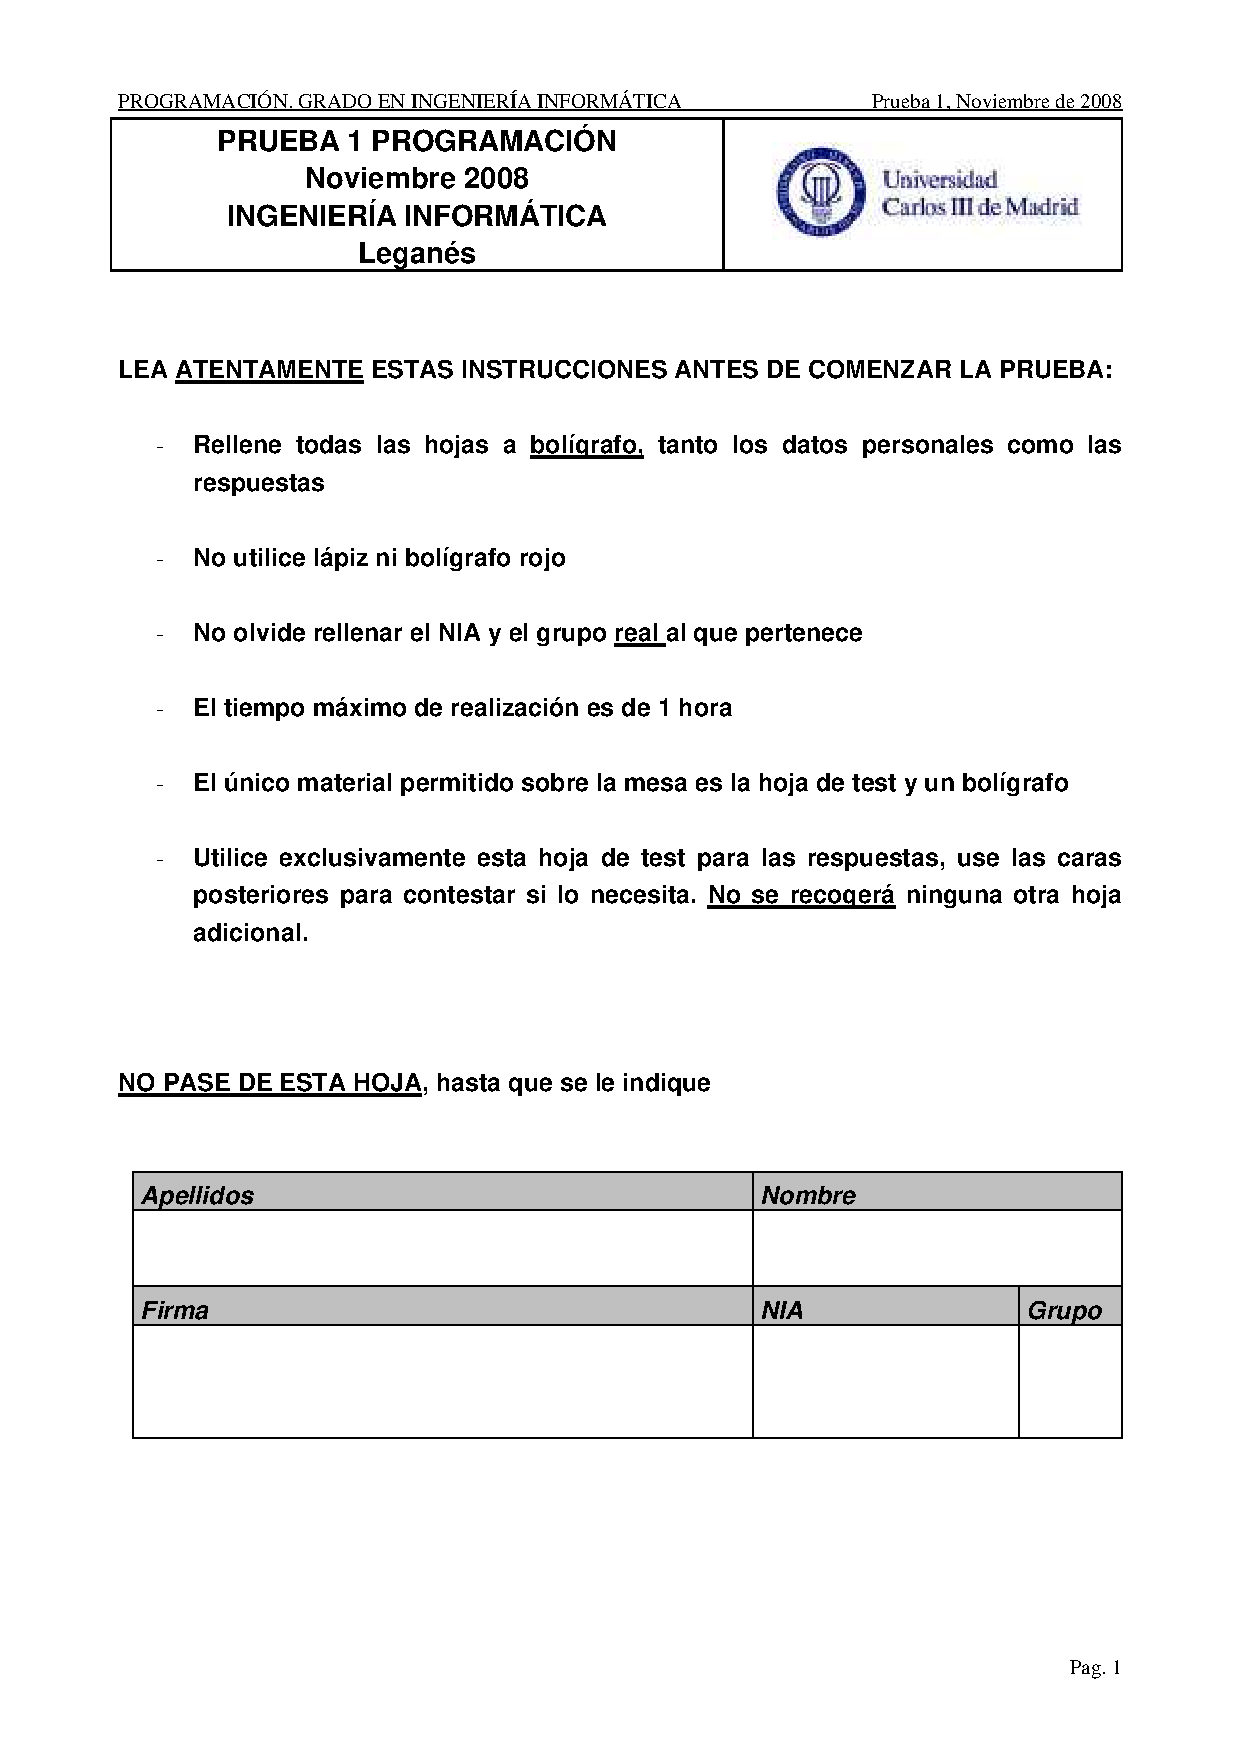
\includepdf[pages=-]{docs/prueba1_nov_08_81L_-_Soluciones.pdf}
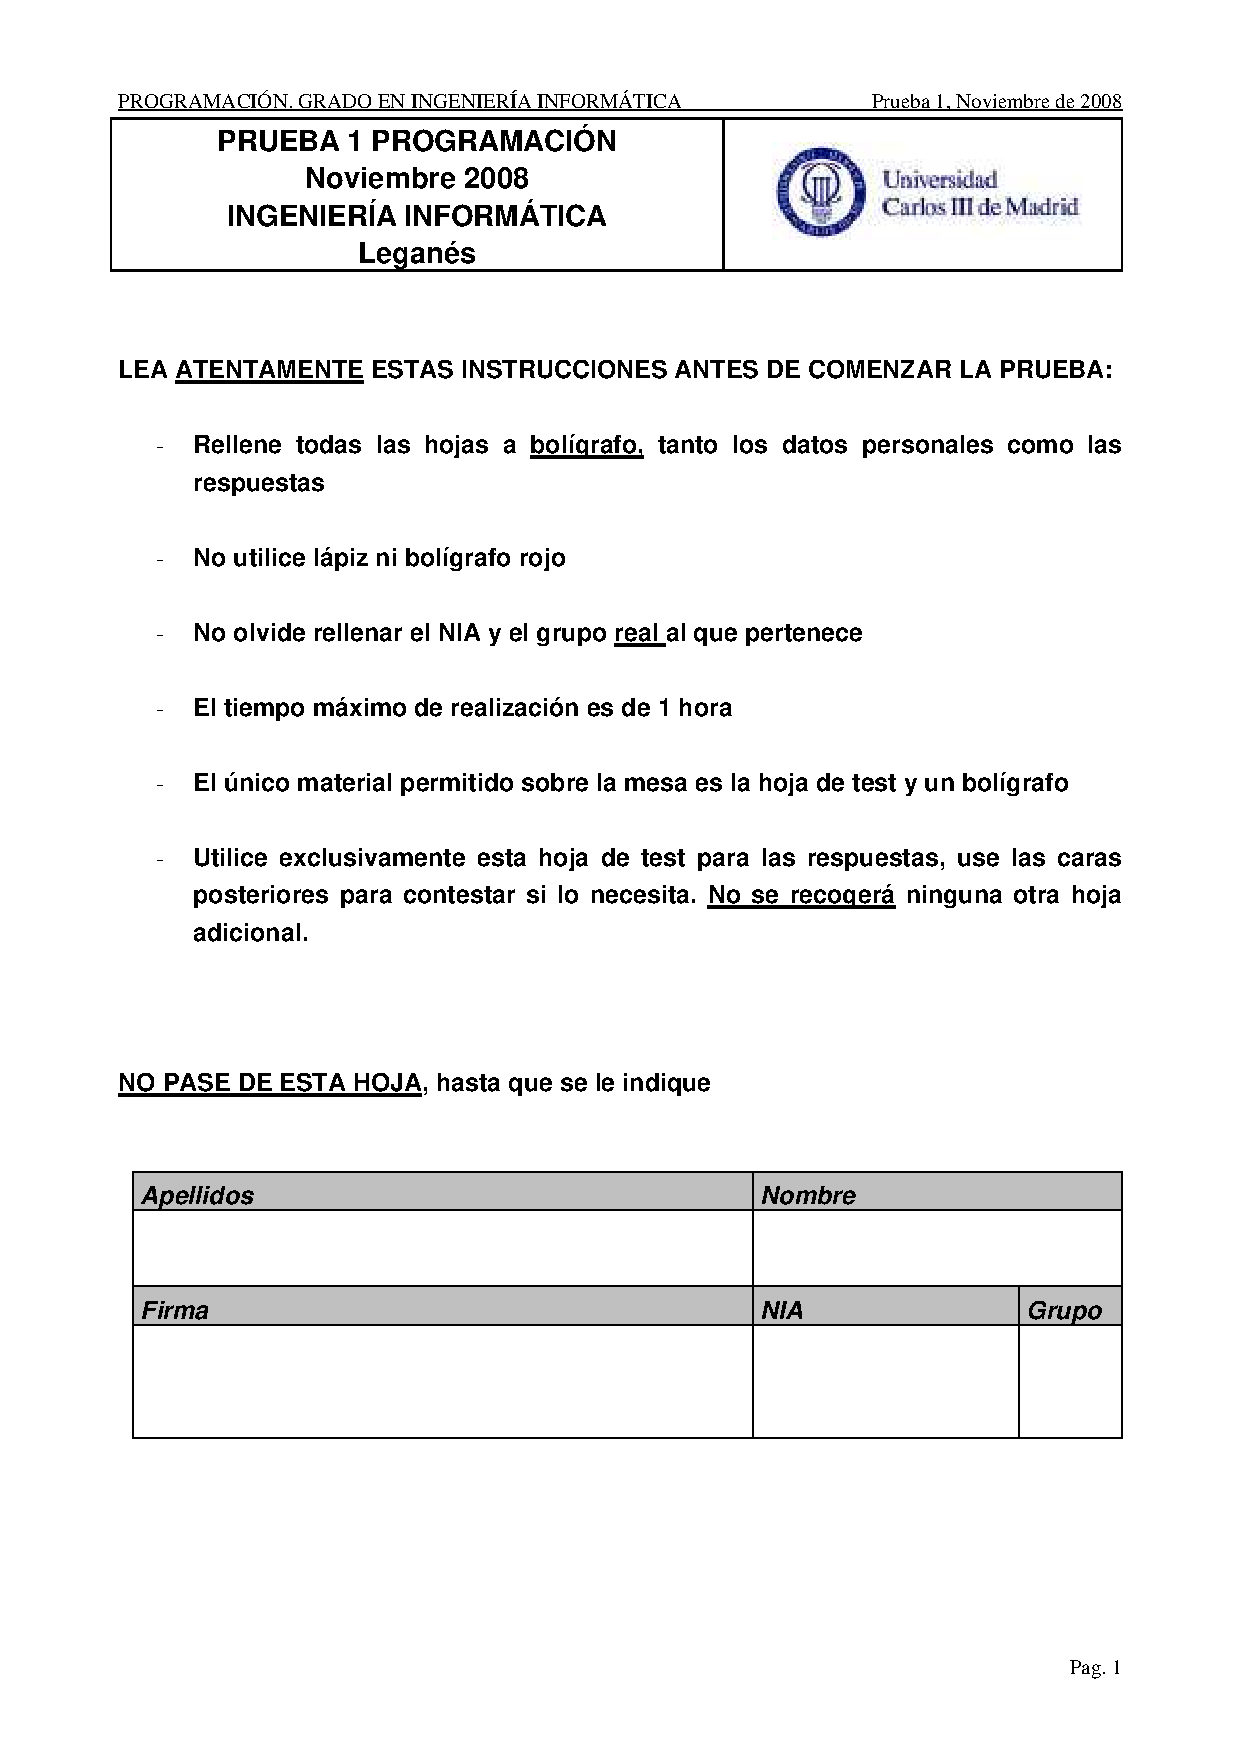
\includepdf[pages=-]{docs/prueba1_nov_08_81L.pdf}
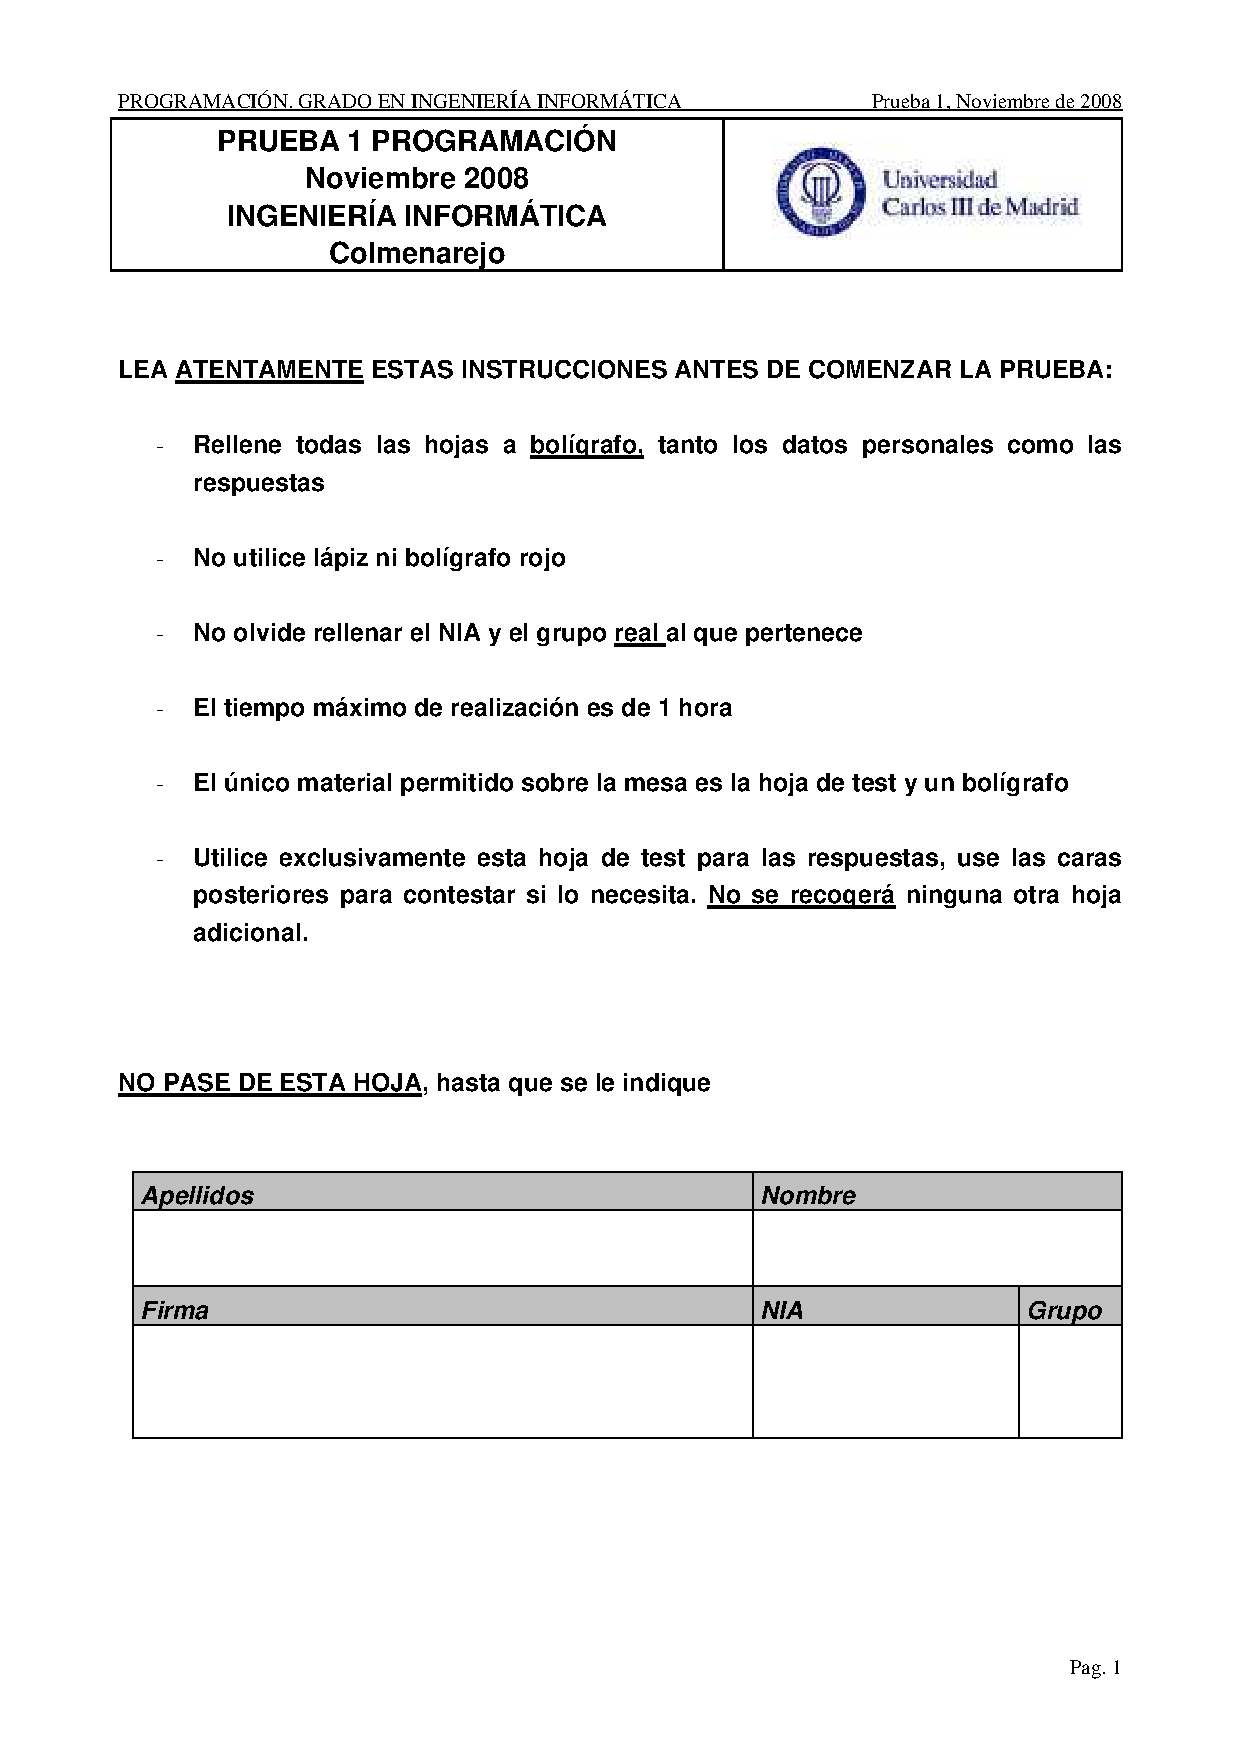
\includepdf[pages=-]{docs/prueba1_nov_08-Colmenarejo-Soluciones.pdf}
\includepdf[pages=-]{docs/prueba1_nov_08-Colmenarejo.pdf}
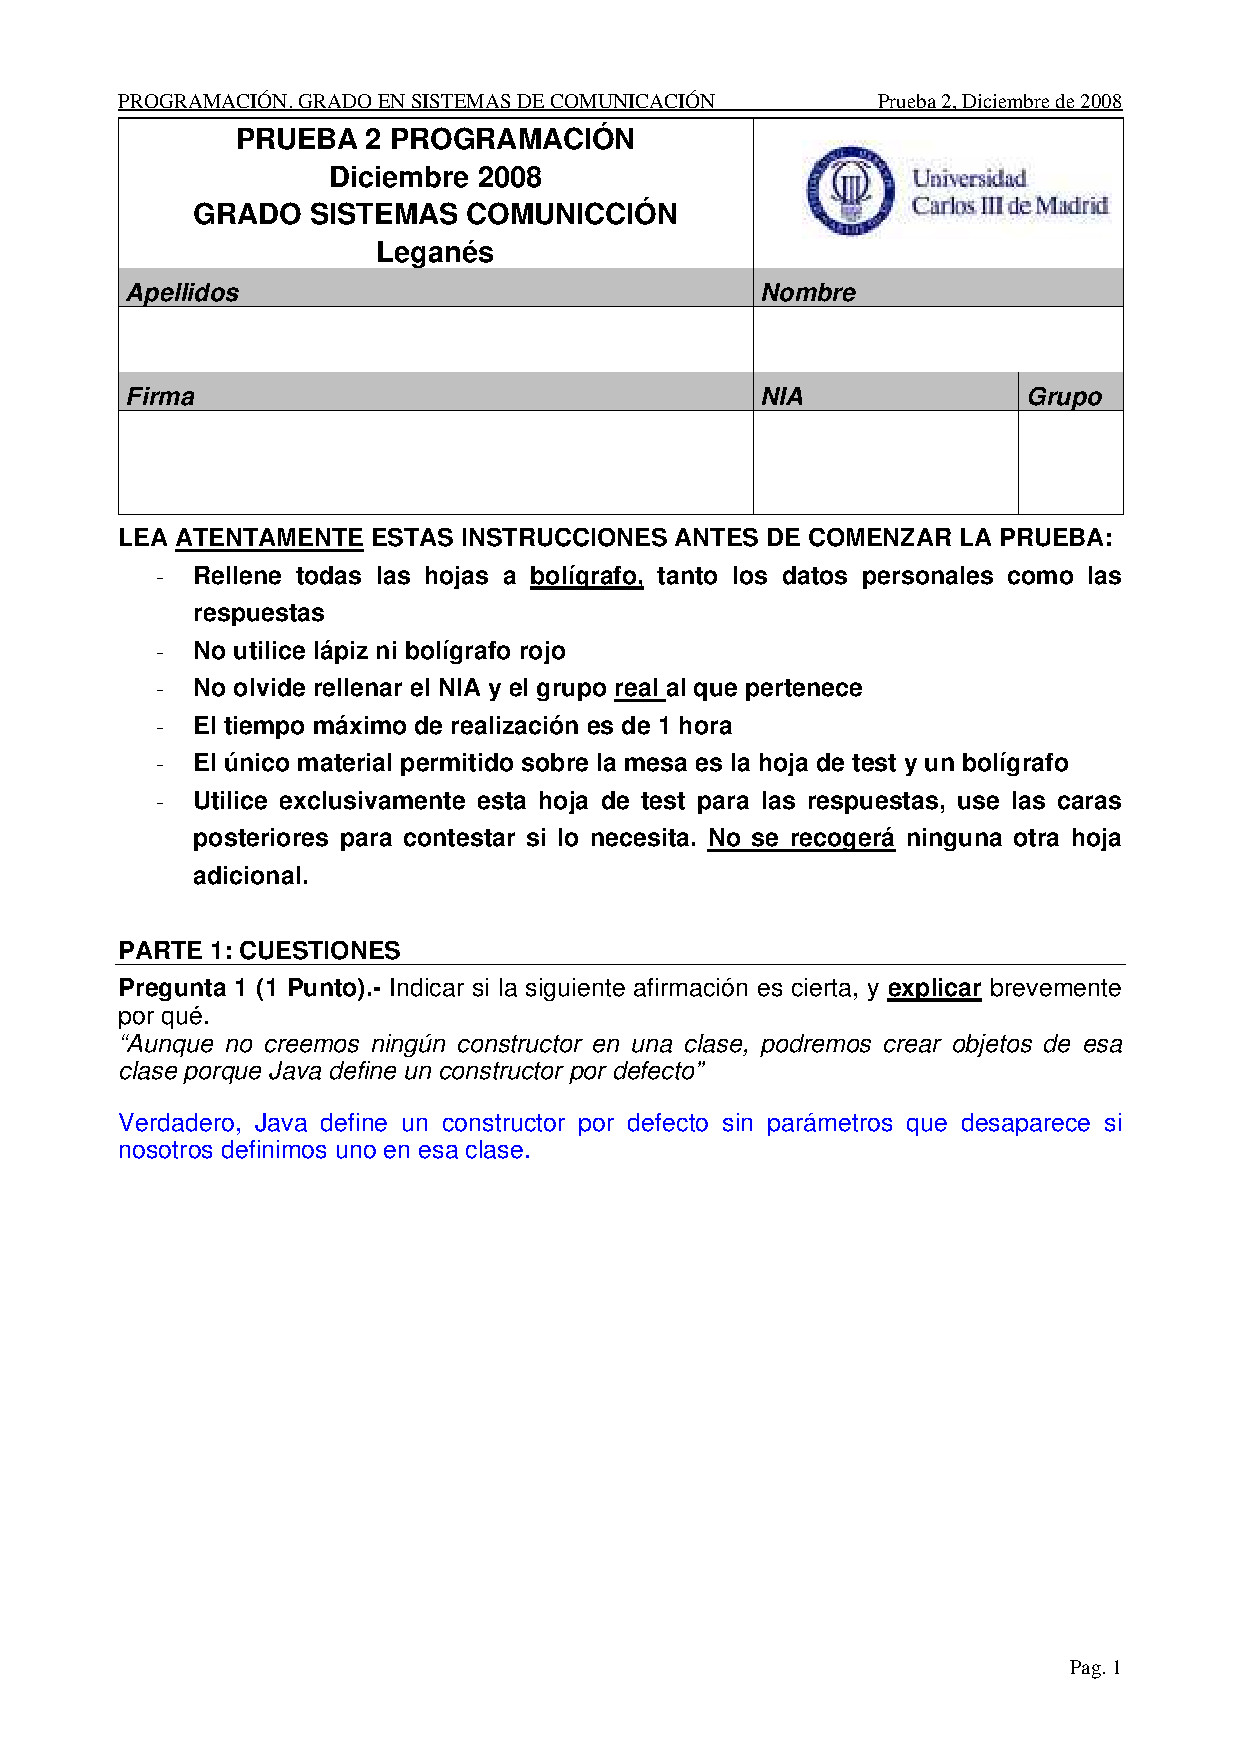
\includepdf[pages=-]{docs/prueba2_dic_08_61-62-Soluciones.pdf}
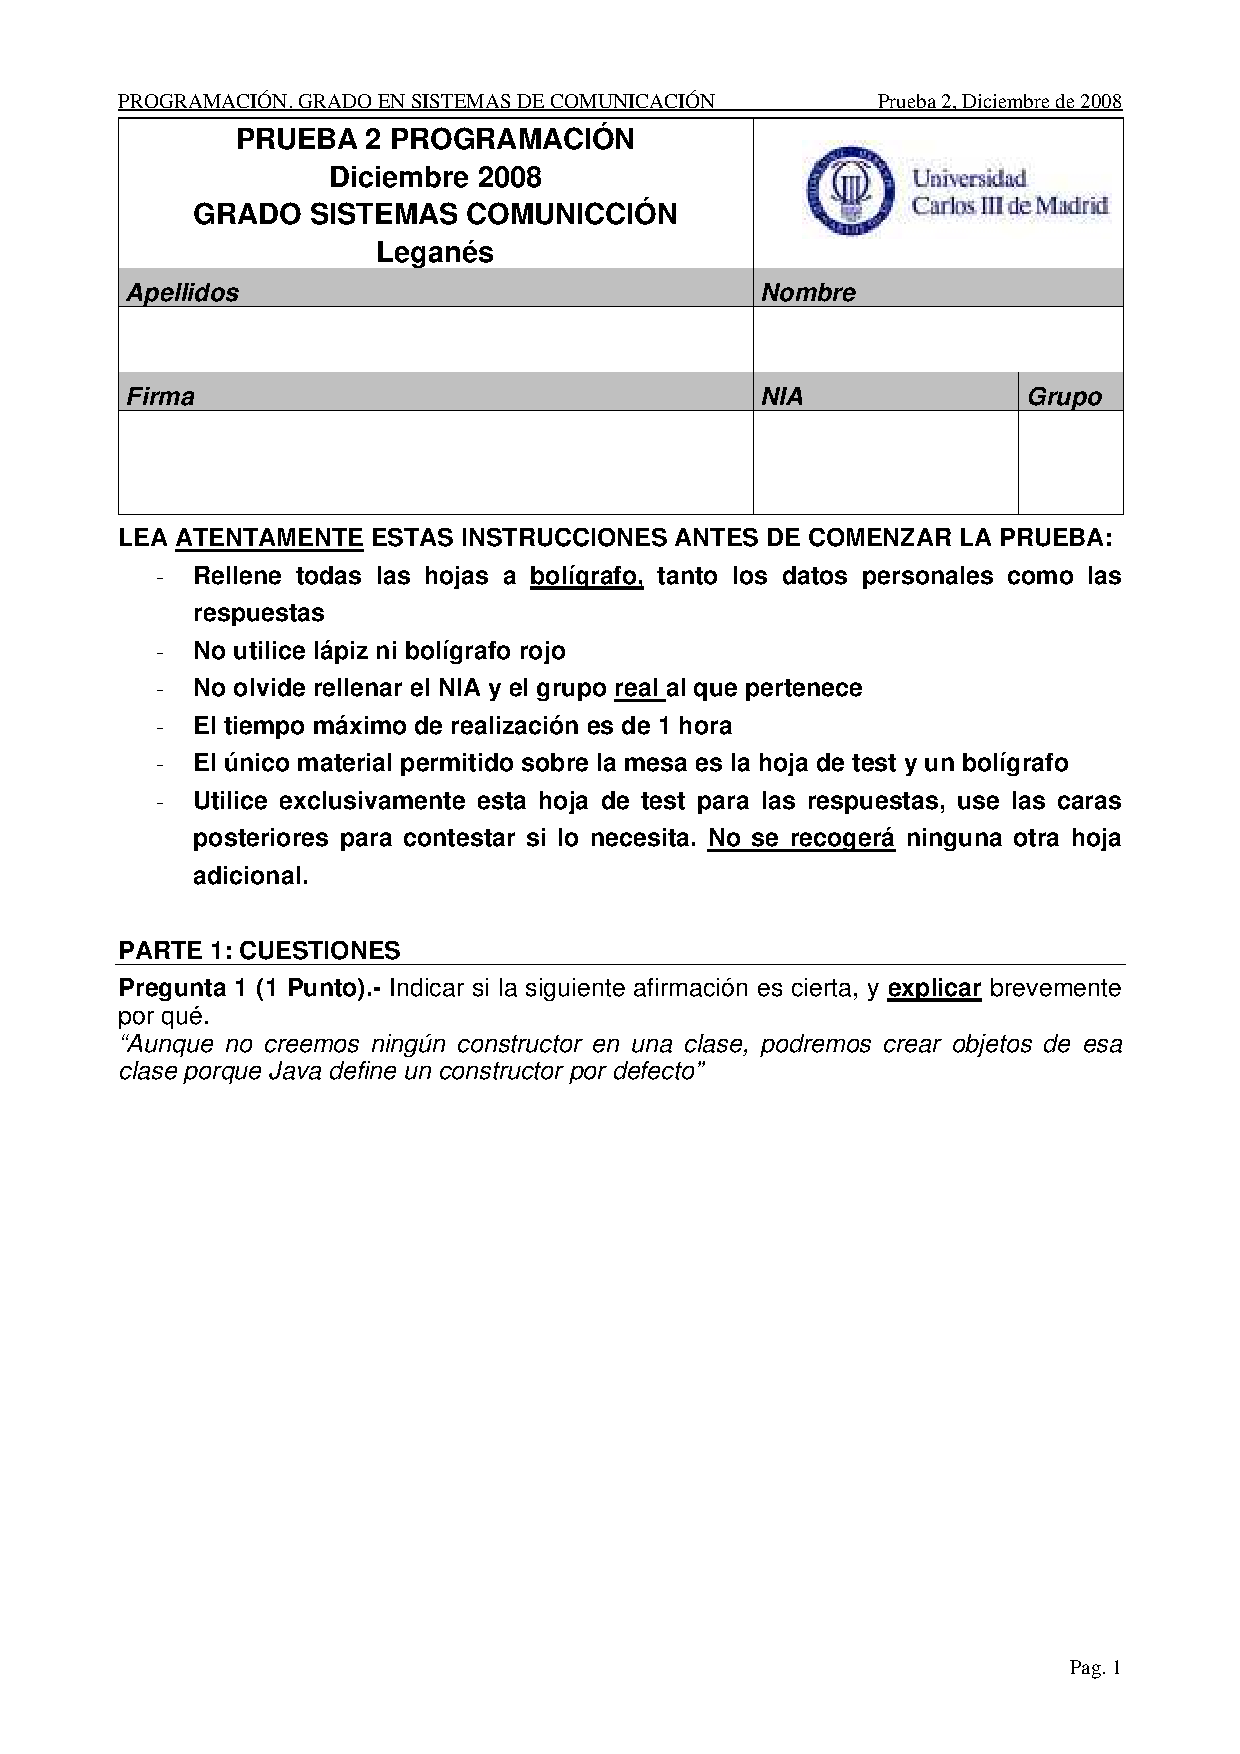
\includepdf[pages=-]{docs/prueba2_dic_08_61-62.pdf}
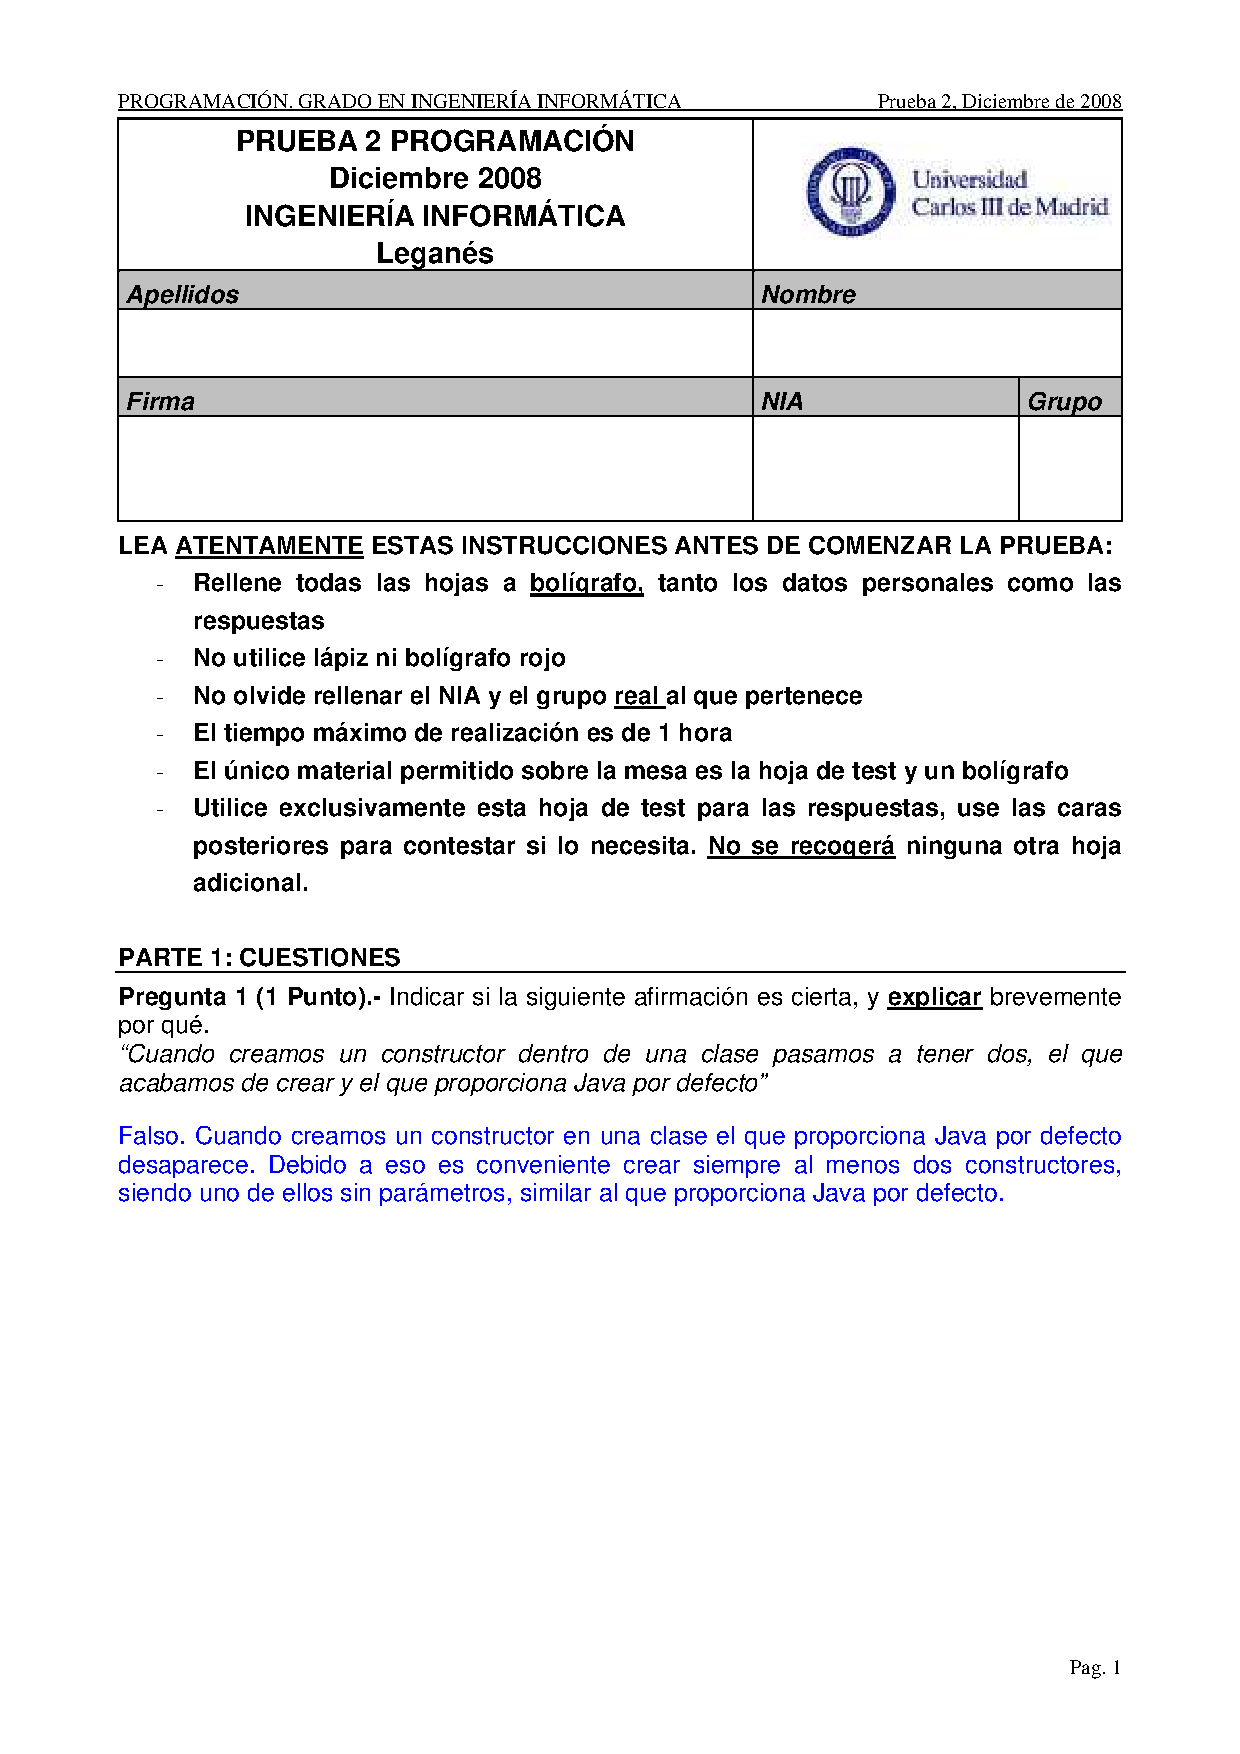
\includepdf[pages=-]{docs/prueba2_dic_08_81L-Soluciones.pdf}
\includepdf[pages=-]{docs/prueba2_dic_08_81L.pdf}
\includepdf[pages=-]{docs/prueba2_dic_08_84L-Soluciones.pdf}
\includepdf[pages=-]{docs/prueba2_dic_08_84L.pdf}
\includepdf[pages=-]{docs/prueba2_dic_08_Colme-Soluciones.pdf}
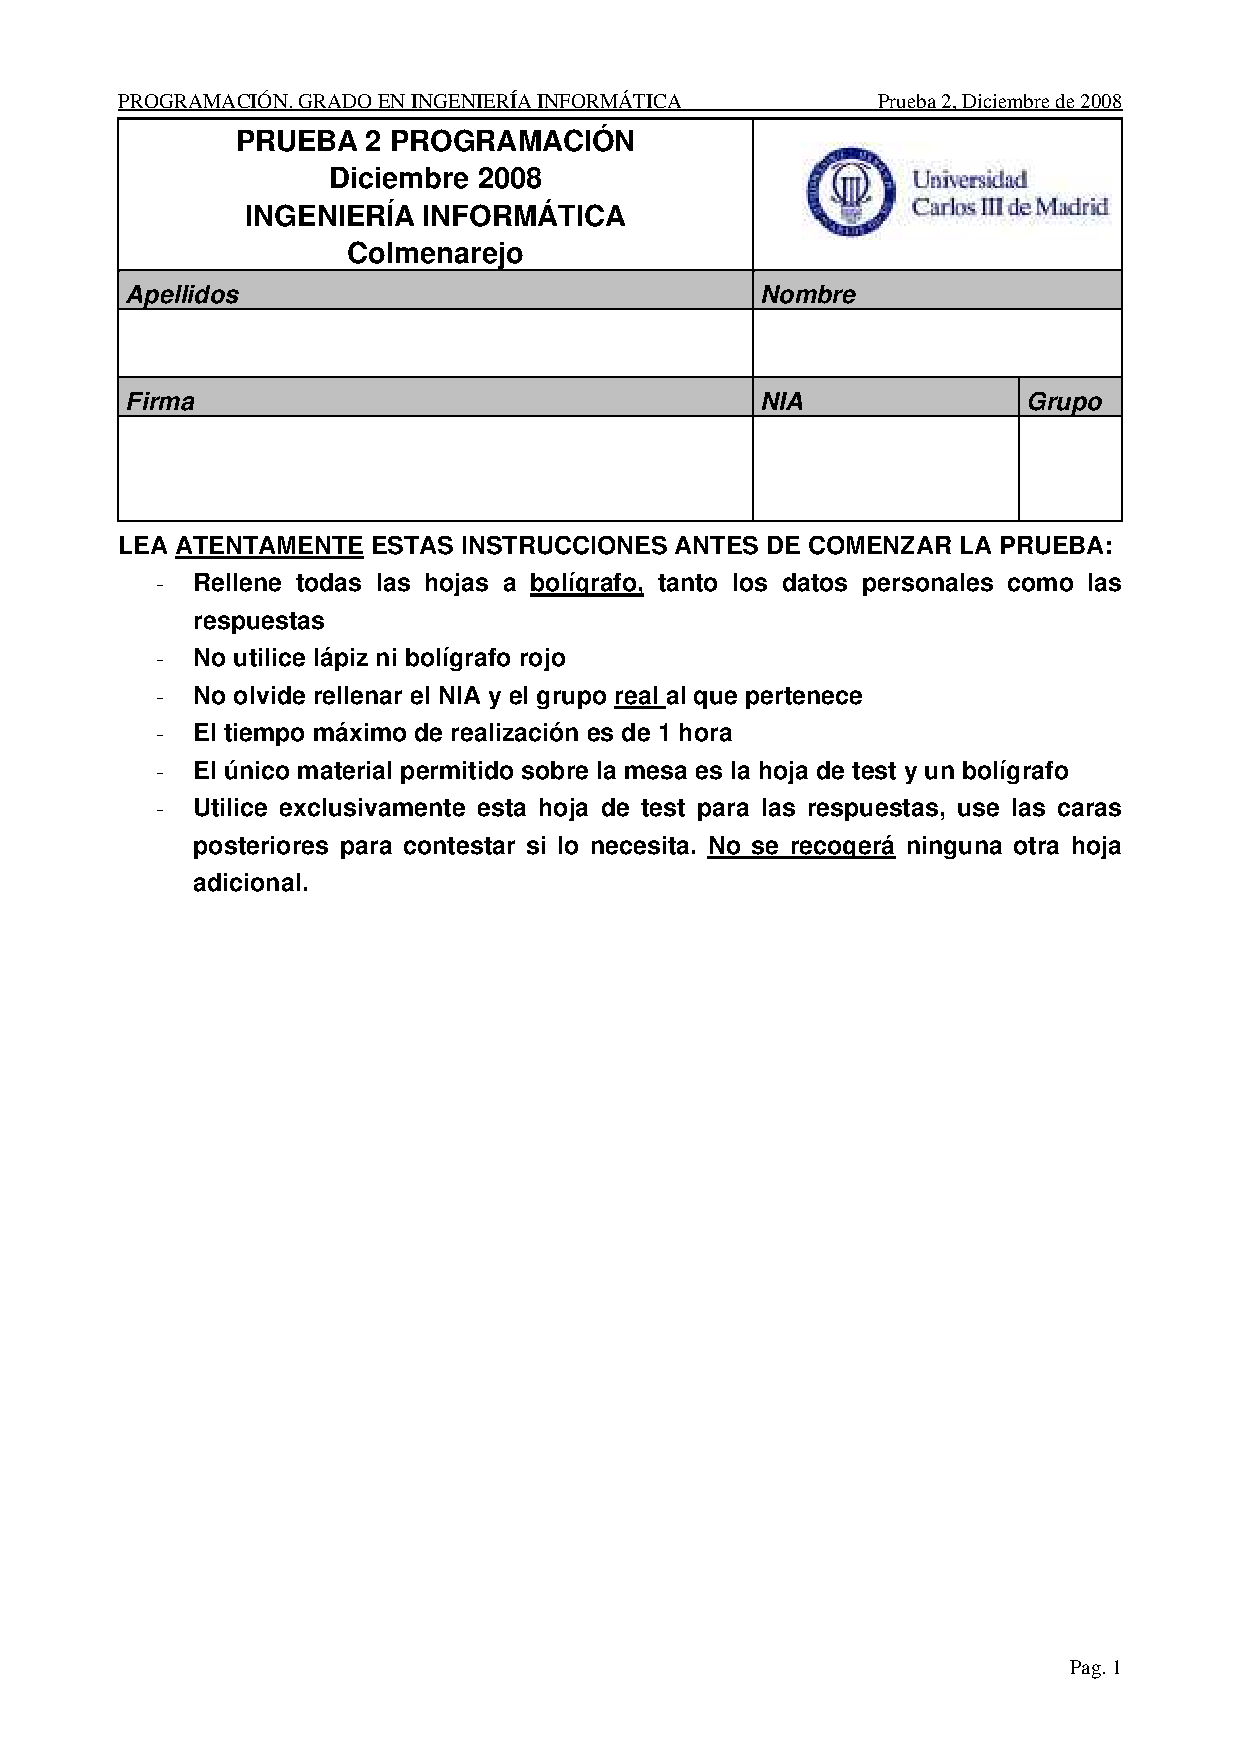
\includepdf[pages=-]{docs/prueba2_dic_08_Colme.pdf}
\includepdf[pages=-]{docs/test1_nov_08_65-Solutions.pdf}
\includepdf[pages=-]{docs/test1_nov_08_89-Solutions.pdf}
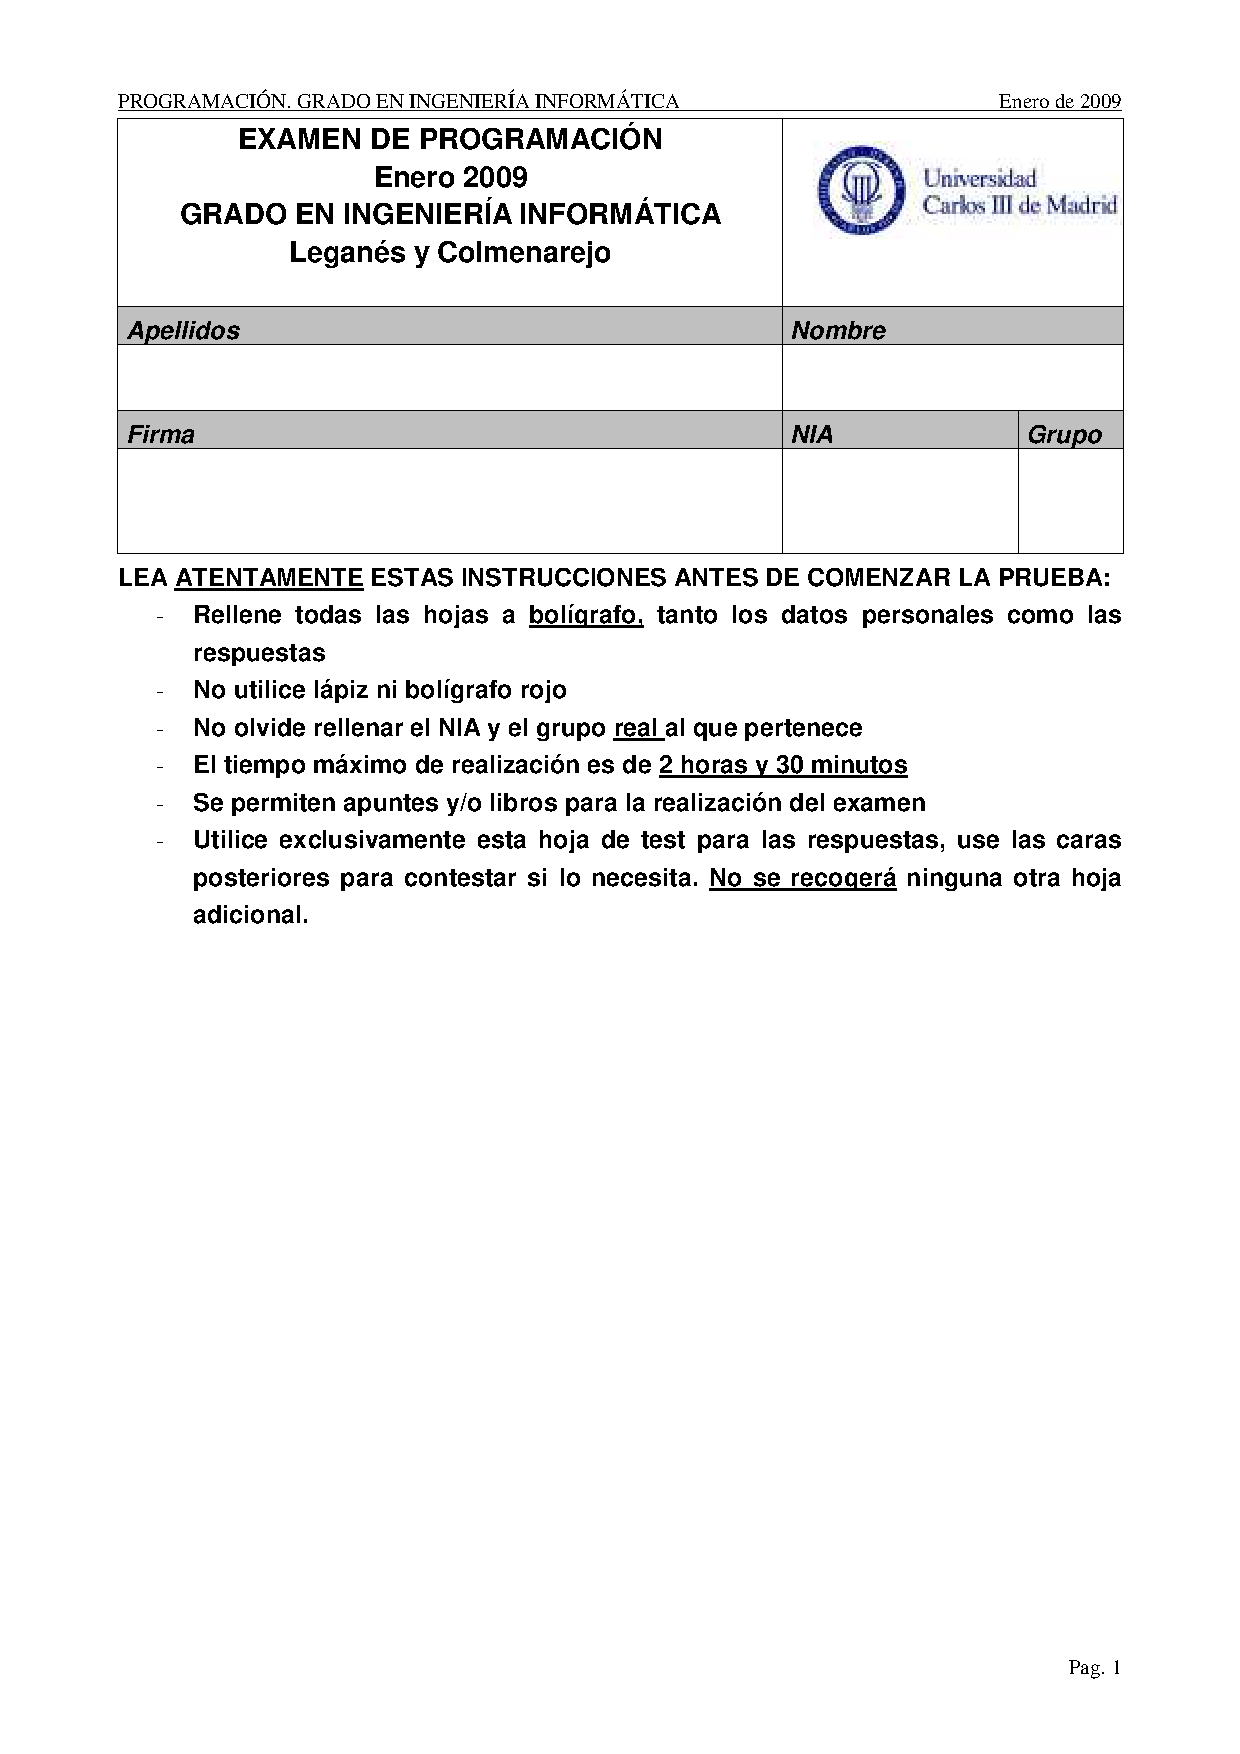
\includepdf[pages=-]{docs/08-09-Enero.pdf}
\includepdf[pages=-]{docs/08-09-Junio.pdf}
\includepdf[pages=-]{docs//09-10-Enero.pdf}
\includepdf[pages=-]{docs/09-10-Junio.pdf}
\includepdf[pages=-]{docs/10-11-Enero.pdf}
\includepdf[pages=-]{docs/10-11-Junio.pdf}
\includepdf[pages=-]{docs/11-12-Enero.pdf}
\includepdf[pages=-]{docs/11-12-Junio.pdf}
\includepdf[pages=-]{docs/11-12-Parcial 1.pdf}
\includepdf[pages=-]{docs/12-13-Enero.pdf}
\includepdf[pages=-]{docs/12-13-Junio.pdf}
\includepdf[pages=-]{docs/13-14-Enero.pdf}
\includepdf[pages=-]{docs/13-14-Junio.pdf}
\includepdf[pages=-]{docs/14-15-Enero.pdf}
\includepdf[pages=-]{docs/14-15-Junio.pdf}
\includepdf[pages=-]{docs/2013_14_ConvOrd_Problemas_Robots_Tesoro.pdf}
\includepdf[pages=-]{docs/exam_dec08a-sol.pdf}
\includepdf[pages=-]{docs/exam_dec08a.pdf}
\includepdf[pages=-]{docs/exam_dec08b-sol.pdf}
\includepdf[pages=-]{docs/exam_dec08b.pdf}
\includepdf[pages=-]{docs/ExamenEneroProgramacion81-85-Soluciones.pdf}
\includepdf[pages=-]{docs/ExamenEneroProgramacion81-85.pdf}
\includepdf[pages=-]{docs/ExJunio2014Programacion-Soluciones.pdf}
\includepdf[pages=-]{docs/Robots_SolucionA.pdf}
\includepdf[pages=-]{docs/Tesoro_solucion.pdf}
\includepdf[pages=-]{docs/200809_P1_autoescuela.pdf}
\includepdf[pages=-]{docs/200809_T1.pdf}
\includepdf[pages=-]{docs/200910_P1_biblioteca.pdf}
\includepdf[pages=-]{docs/200910_T1.pdf}
\includepdf[pages=-]{docs/200910_T2.pdf}
\includepdf[pages=-]{docs/EjerciciosExtra_es.pdf}
\includepdf[pages=-]{docs/EjerciciosExtra2_es.pdf}

\end{document}